
\section{Experiments}
\label{sec:experiments}

\subsection{Experimental Setup}

We evaluate \methodname{} against Interp3D~\cite{liu2026interp3d} and MorphAny3D~\cite{sun2026morphany3d} on 50 held-out source pairs. To ensure a controlled comparison, all methods use identical endpoint SLat representations generated by TRELLIS~\cite{xiang2025trellis} with the same code, configuration, and random seeds. All generated assets are evaluated using a common Gaussian renderer with matched cameras.

We adopt the Interp Protocol of Interp3D, consisting of five intermediates sampled at deterministic $\operatorname{Beta}(5,5)$ quantiles and two canonical endpoints. We additionally use the Dense Protocol \citep{sun2026morphany3d} with 48 uniformly spaced intermediates at $t=k/49$, yielding 50 states including the endpoints. LPIPS-based distances are evaluated over 64 matched views, while FID uses 1,000 views per state and two intermediate states selected identically for all methods. FID, PPL, and PDV follow the Interp Protocol, whereas EPRE is evaluated under both protocols. This evaluation applies the Interp3D protocol to our held-out pairs rather than reproducing the Interp3DData leaderboard.

\subsection{Quantitative Results}

\begin{table*}[t]
\centering
\small
\setlength{\tabcolsep}{3pt}
\caption{Comparison on 50 held-out pairs. Values are means; \textbf{bold} and \underline{underline} mark the best and second mean in each column. FID, PPL, LPIPS, and PDV use the Interp Protocol; EPRE and TIME report both protocols. LPIPS, PPL, PDV, and EPRE include canonical endpoints. FID uses the concatenated-state definition. PDV is reported in units of $10^{-3}$. TIME is generation time per sequence in seconds. All metrics are minimized.}
\label{tab:standard}
\begin{tabular}{lrrrrrrrr}
\toprule
Method & FID $\downarrow$ & PPL $\downarrow$ & LPIPS $\downarrow$ & PDV ($10^{-3}$) $\downarrow$ & \multicolumn{2}{c}{EPRE $\downarrow$} & \multicolumn{2}{c}{TIME (s) $\downarrow$} \\
\cmidrule(lr){6-7}\cmidrule(lr){8-9}
& & & & & Interp Protocol & Dense Protocol & Interp Protocol & Dense Protocol \\
\midrule
MorphAny3D & \second{95.95} & \best{2.87} & \best{0.118} & $4.88$ & $0.33$ & $0.39$ & \second{182} & $1914$ \\
Interp3D & $96.02$ & \second{3.31} & \second{0.137} & \second{1.40} & \second{0.27} & \second{0.35} & $188$ & \second{897} \\
\methodname{} (ours) & \best{95.03} & $3.58$ & $0.148$ & \best{0.85} & \best{0.26} & \best{0.32} & \best{61} & \best{553} \\
\bottomrule
\end{tabular}
\end{table*}


Table~\ref{tab:standard} compares the three methods in terms of intermediate quality, perceptual path properties, endpoint progression, and computational efficiency. All methods achieve comparable FID scores, with \methodname{} obtaining the lowest value. Although our method has a higher PPL, indicating a longer perceptual path, it achieves the lowest PDV, reducing it by 39\% compared to Interp3D. This suggests that our method distributes perceptual changes more uniformly along the transition, despite traversing a longer path. In contrast, shorter perceptual paths do not necessarily imply more regular transitions.

Our method also achieves the lowest EPRE under both evaluation protocols, indicating closer agreement with the reference endpoint progression. The improvement is particularly evident under the Dense Protocol, where EPRE decreases from 0.35 for Interp3D to 0.32 for our method. Figure~\ref{fig:epre_profile} provides a more detailed analysis, showing that our method generally produces lower profile errors, particularly near the endpoints, while remaining comparable to Interp3D around the midpoint.

\begin{figure}[t]
    \centering
    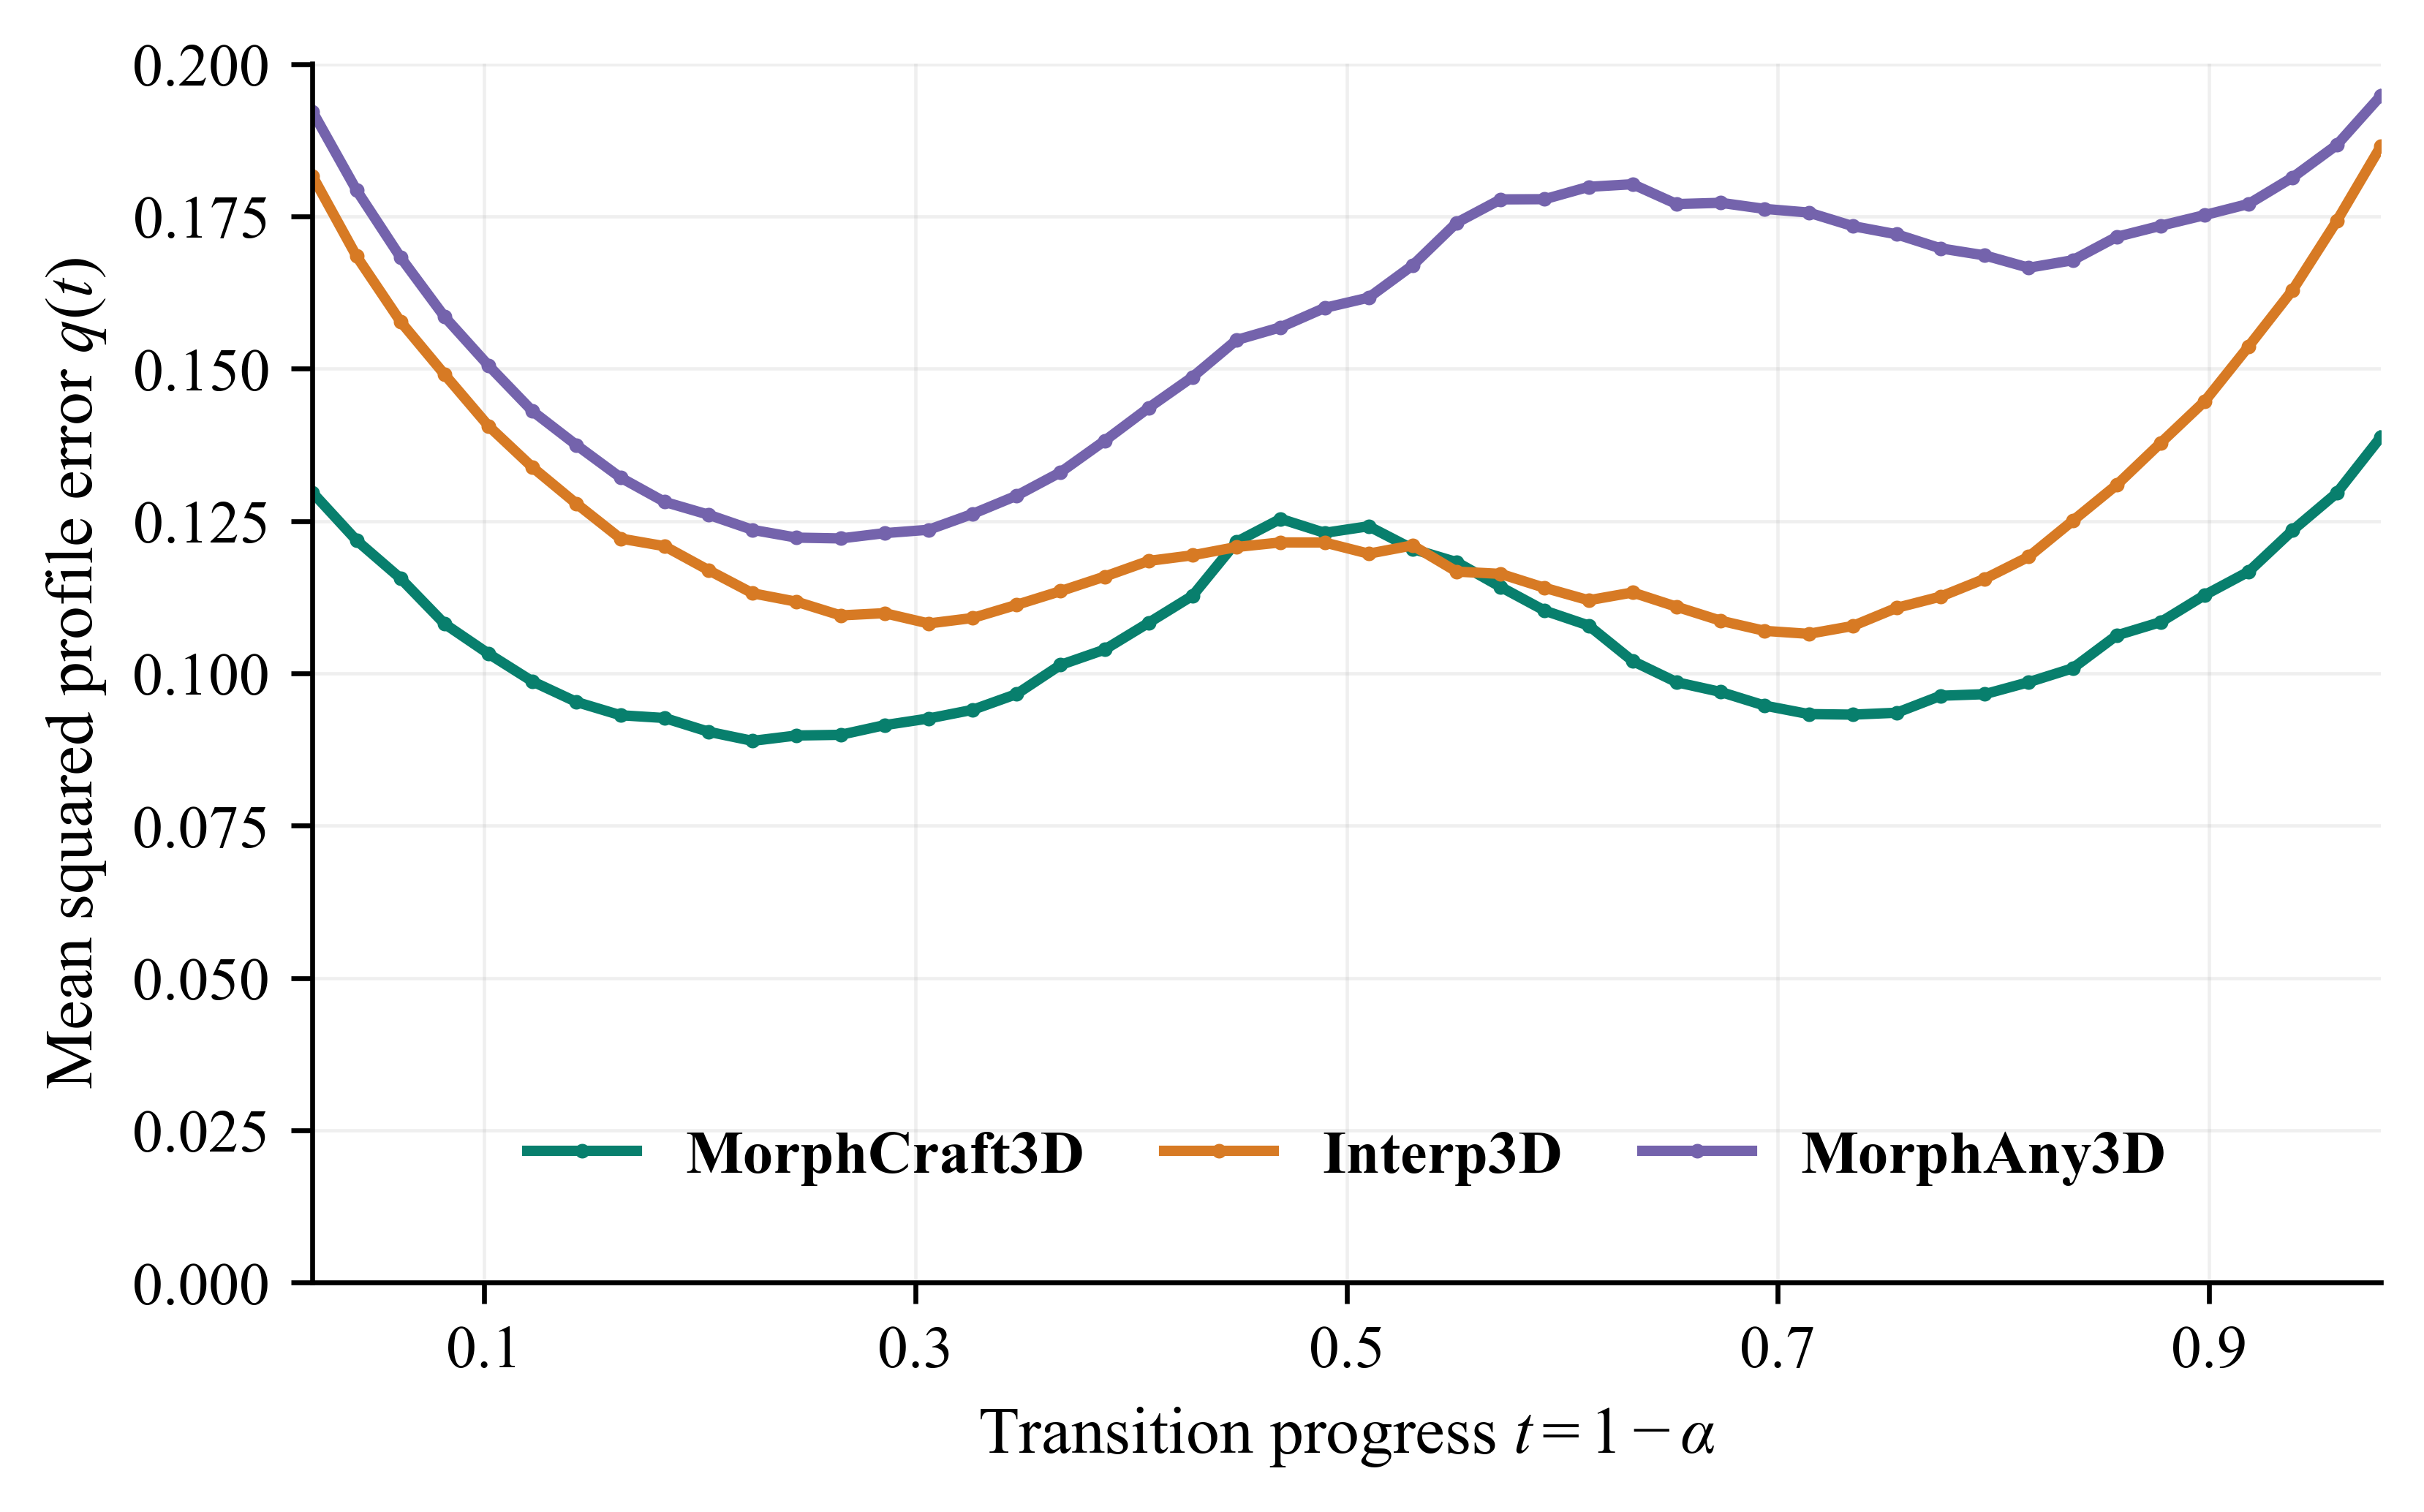
\includegraphics[width=\columnwidth]{figures/epre.png}
    \caption{\textbf{Instantaneous squared endpoint profile error.}
    Mean $q(t)$ over 50 pairs.  Lower values indicate closer agreement with the linear reference.}
    \label{fig:epre_profile}
\end{figure}

Finally, \methodname{} achieves the lowest measured generation time under both protocols. Under the Interp Protocol, it requires 61 seconds per sequence, compared to 188 seconds for Interp3D and 182 seconds for MorphAny3D. The advantage remains under the Dense Protocol, where our method requires 553 seconds compared to 897 and 1914 seconds, respectively.

\subsection{Qualitative Results}

\subsection{Ablation Studies}
\label{sec:ablations}


% \section{Experiments}
% \label{sec:experiments}

% The comparison uses the same 50  source pairs, and a common Gaussian renderer with matched cameras. The
% Interp Protocol follows Interp3D and contains seven states: two canonical sources and five
% intermediates at deterministic $\operatorname{Beta}(5,5)$ quantiles.
% LPIPS uses 64 views; FID uses 1,000 views per state and two intermediate
% states selected identically for all methods. The Dense Protocol generates
% 48 uniform intermediates at $t=k/49$, for 50 states in total, to resolve
% behavior near the endpoints. Only EPRE and generation time are available
% for the Dense Protocol. This evaluates the teacher protocol on our
% pairs, rather than reproducing the Interp3DData leaderboard.

% \subsection{Comparison}
% Table~\ref{tab:standard} compares \methodname{},
% MorphAny3D~\cite{sun2026morphany3d}, and Interp3D~\cite{liu2026interp3d}.
% The methods obtain similar FID means. \methodname{} has lower PDV but a
% longer perceptual path, indicating more uniform step magnitudes while
% traversing a greater total distance. Under the Dense Protocol it obtains
% the lowest mean EPRE. Generation time includes preparation and raw-asset
% serialization, excluding one-time model loading and metric rendering.

% Figure~\ref{fig:distances50} shows how each method moves away from one
% source and approaches the other. Reading both distances together
% distinguishes a transition that stays close to one source from one that
% departs from both. Figure~\ref{fig:qualitative} complements these averages
% with matched views of geometry and appearance.

% \begin{figure*}[t]
%  \centering
%  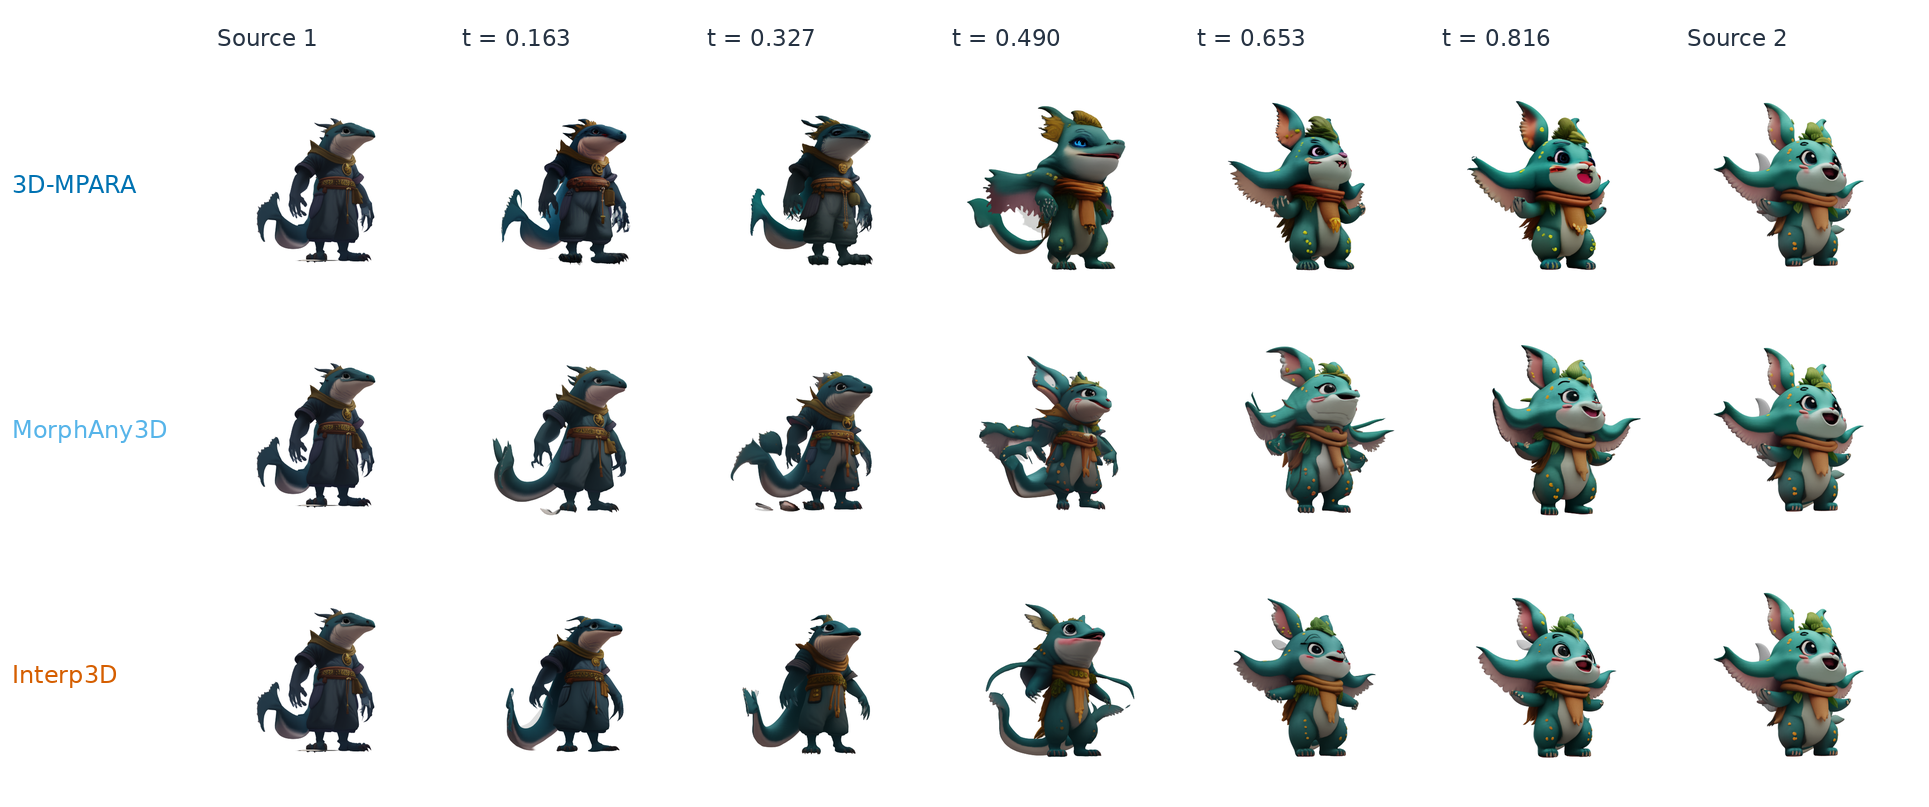
\includegraphics[width=.94\textwidth]{figures/qualitative_pair_0000.png}\\[3pt]
%  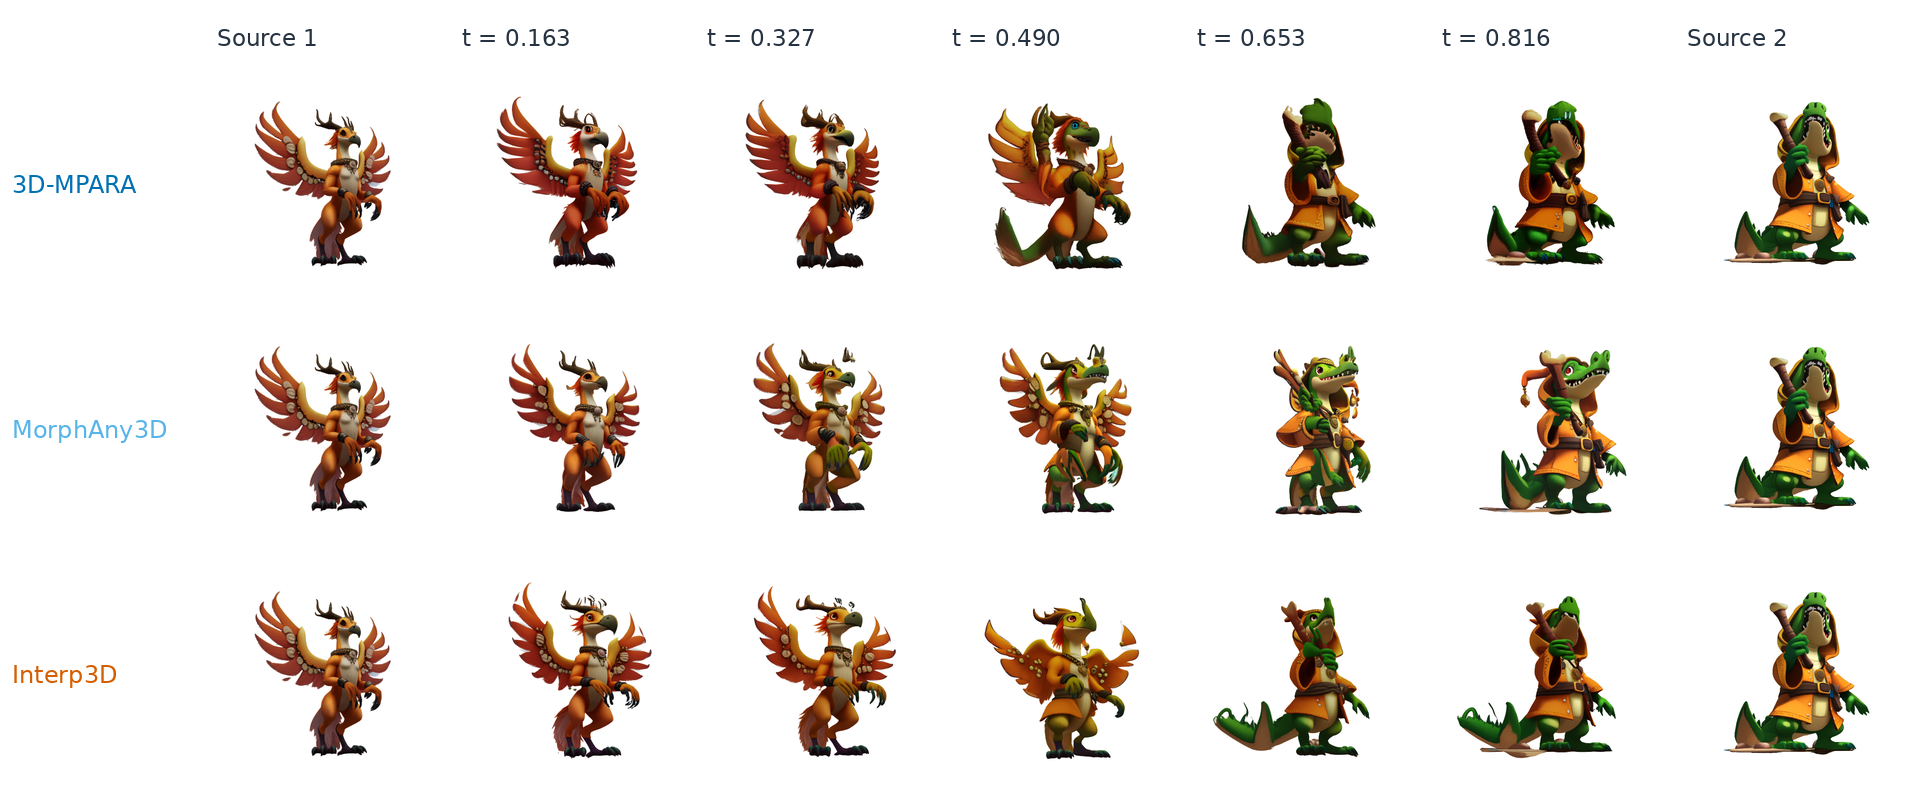
\includegraphics[width=.94\textwidth]{figures/qualitative_pair_0001.png}
%  \caption{\textbf{Textured morphing comparisons.} Each pair has one row per
%  method and a fixed camera (view 025). Columns show seven samples from the
%  dense sequences at $t=0,8/49,16/49,24/49,32/49,40/49,1$.
%  Sources are common canonical assets. These are the first two pairs in
%  the test plan, selected without metric ranking.}
%  \label{fig:qualitative}
% \end{figure*}

% \begin{figure}[h]
%  \centering
%  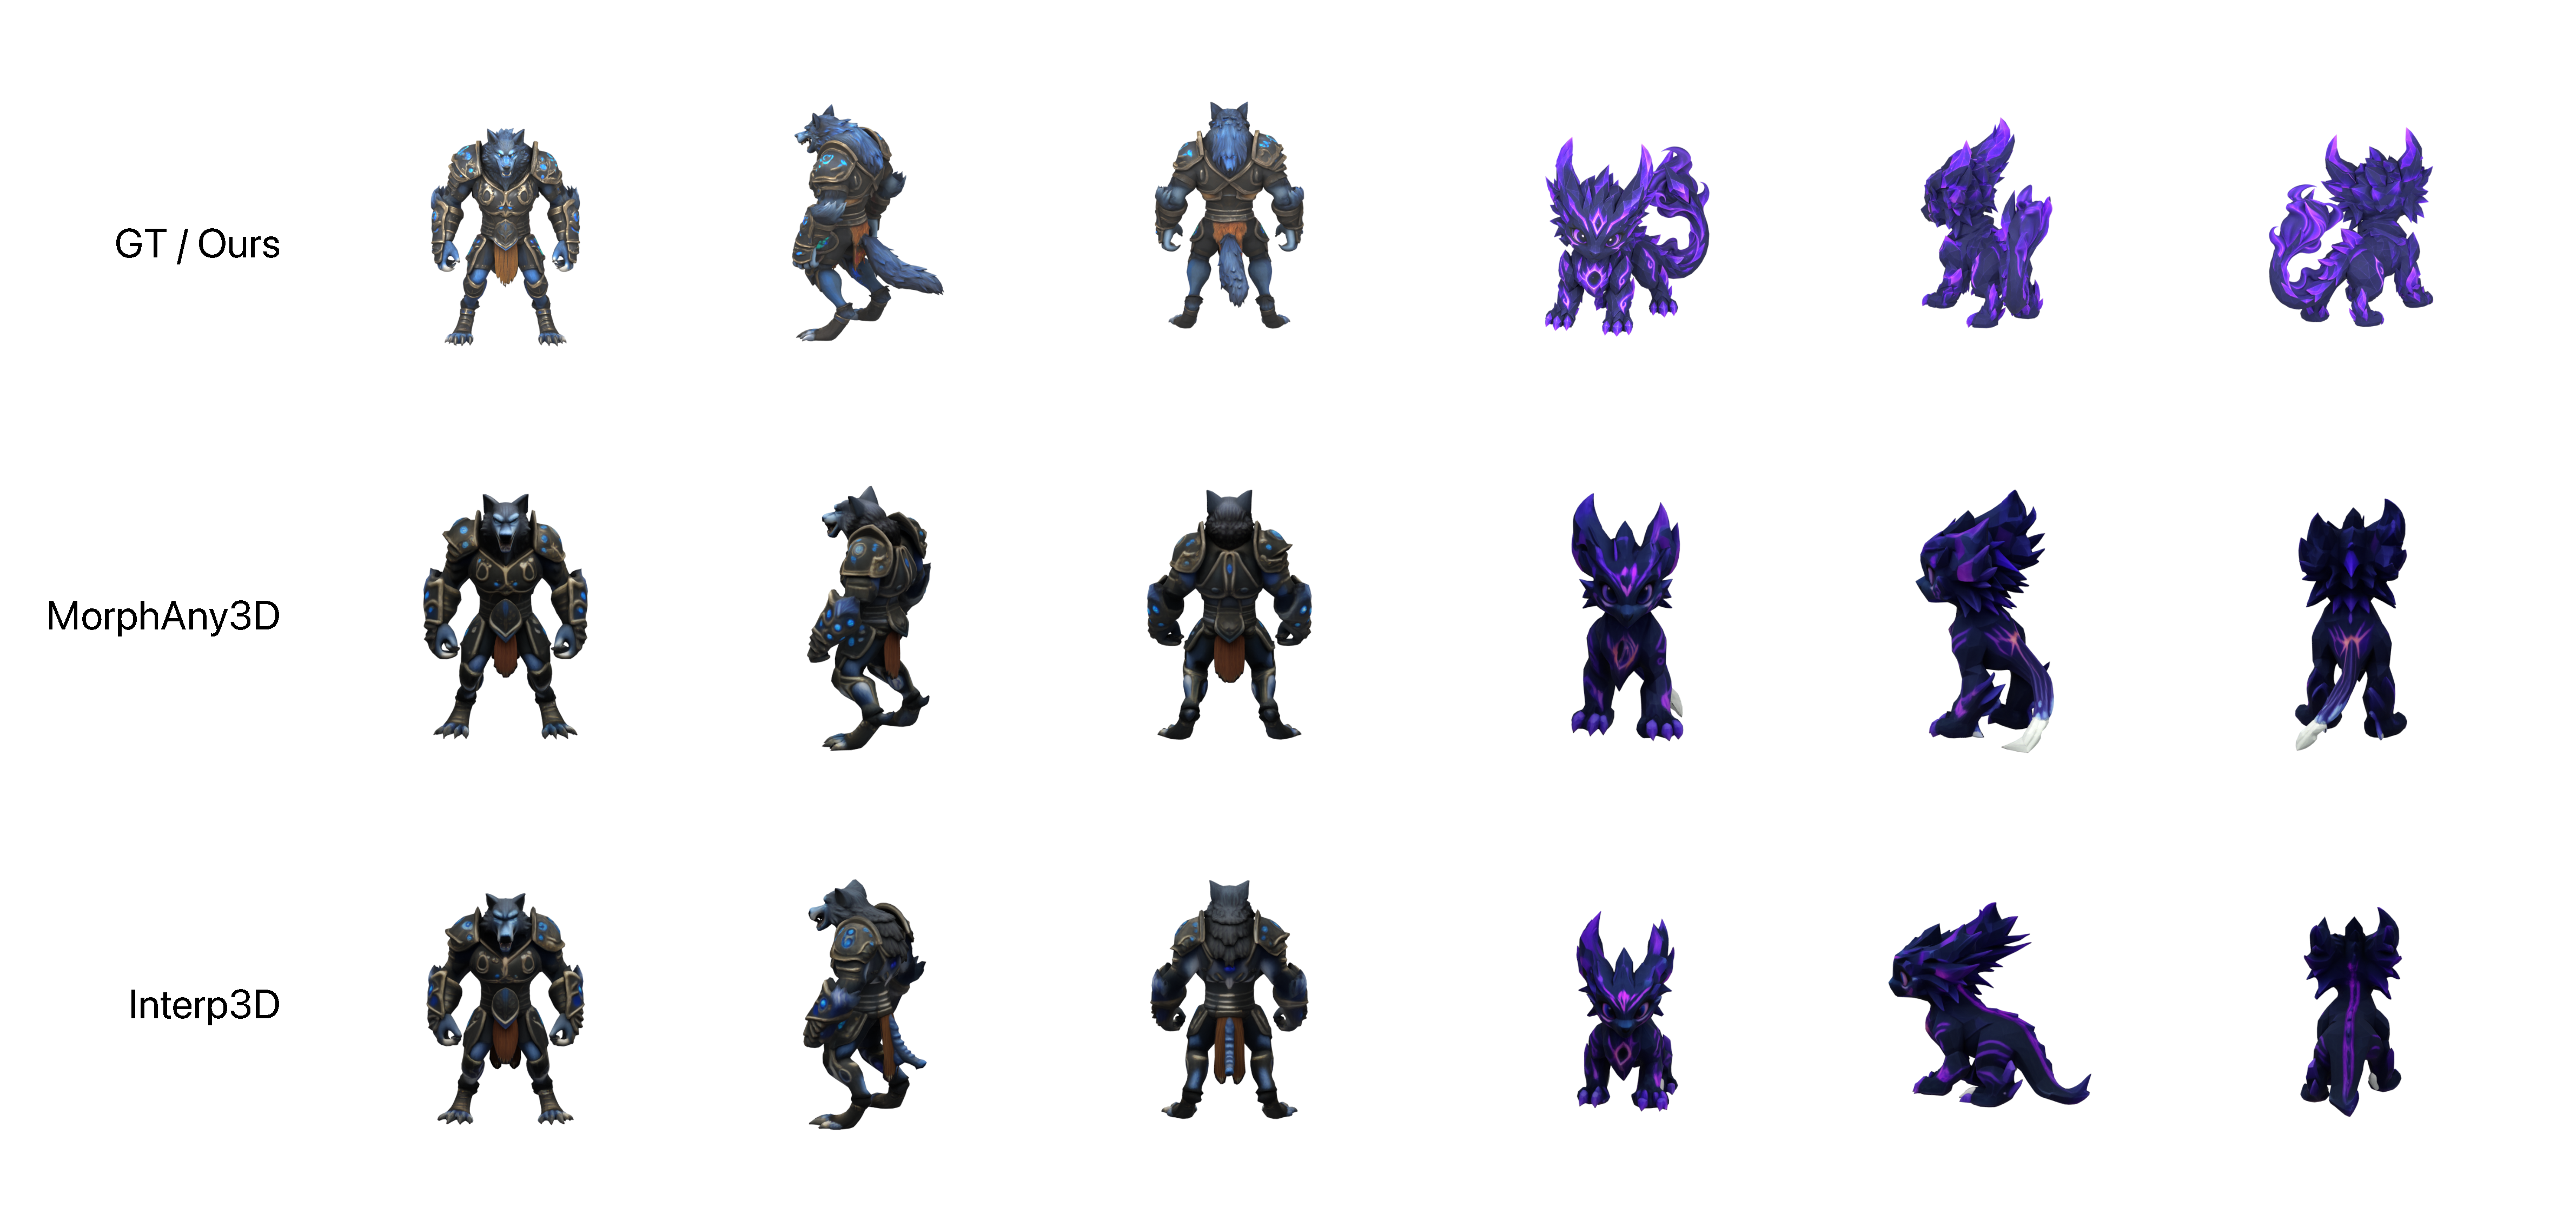
\includegraphics[width=\columnwidth]{figures/comparison_errors.pdf}
%  \caption{todo}
%  \label{fig:comparison_errors}
% \end{figure}


% \subsection{Ablations}
% \label{sec:ablations}

% The ablation study uses the Interp Protocol to test whether the prior improves FID and
% gating reduces PDV. The full model targets a balance between source
% fidelity and transition quality. Table~\ref{tab:ablation} awaits
% matched-step results.

% \begin{table}[t]
\centering
\small
\setlength{\tabcolsep}{5pt}
\caption{Ablations under the Interp Protocol. Baseline disables gate, prior, and source swap; component variants enable only the named term, and Full Model uses all three. Final matched-step measurements are pending.}
\label{tab:ablation}
\begin{tabular}{lrrrr}
\toprule
Variant & FID $\downarrow$ & PPL $\downarrow$ & PDV $\times10^3\!\downarrow$ & EPRE $\downarrow$ \\
\midrule
Baseline & 96.54 & \second{3.55} & 0.90 & 0.26 \\
Gate Only & 102.34 & \best{3.54} & \best{0.84} & 0.26 \\
Prior Only & \best{91.17} & 3.58 & 0.91 & 0.26 \\
Full Model & \second{95.03} & 3.58 & \second{0.85} & 0.26 \\
\bottomrule
\end{tabular}
\end{table}

